% !TeX root = dissertation.tex
\chapter{CPU virtualization}
\label{sec:cpuvirt}
In order to understand CPU Virtualization as it is today, it is illuminating
to consider the history of the technique, even though a complete treatment of
this subject is out of the scope of this proposal (interested readers are
instead referred to Bugnion, Nieh, and Tsafrir's book on this topic---\emph{
Hardware and software support for virtualization}~\cite{bugnion-nieh-tsafrir}.)

CPU virtualization as a technique was first considered for the IBM 360 in 1970~
\cite{meyer-virtual-machines}. The idea then, as it is today is, was to provide
each user with the illusion of having a dedicated machine to themselves, by
simultaneously running multiple operating systems on the same machine.
The IBM~370 was specifically designed to be \emph{virtualizable}~\cite{vm370},
while a concurrent machine, the PDP-10, wasn't. The inability to virtualize
the PDP-10 led Popek and Goldberg~\cite{popek-goldberg} to formalize the
requirements of a Virtual Machine Monitor---\emph{equivalence, safety, and
performance}---and three theorems about the virtualizability of an Instruction
Set Architecture (ISA). To summarize briefly, a VMM or a hypervisor must meet
the following criteria:
the virtual machine constructed by the VMM must be indistinguishable from the
native machine (equivalence), must not be able to access resources not
allocated to it or influence the way these resources are used by other VMs or
the hypervisor (safety), and the performance of software executing in the VM
must be comparable to native (performance).
The first theorem defined what it means for an ISA to be virtualizable.
The second theorem was concerned with recursive or nested virtualization.
The third theorem presents the necessary conditions for a \emph{Hybrid Virtual
Machine}---one that combines direct execution of non-sensitive instructions
with emulation for all sensitive instructions----to be designed for ISAs that
violate the first theorem.

While virtualization was well understood and in production in the 1970s, all
the lessons learned during that time were seemingly lost or ignored by later
computer architects. The new ISAs that established their dominance in
computing as the mainframe computers of the 1970s were rendered mostly
obsolete by the Personal Computer (Intel x86, DEC ALPHA, SUN SPARC, IBM POWER,
MIPS, ARM, etc.) were all unvirtualizable. Even though some of them initially
supported virtualizable modes, (e.g., Intel x86's 16-bit virtual mode---
\texttt{v8086}---allowed the execution of 16-bit software in 32-bit mode.),
this support was left on the wayside as the ISA evolved. Virtualization was
considered a quirky bad idea from the 1970s.

Hardware virtualization made a come back in the late 1990s and early
2000s~\cite{bugnion-disco, denali, xen} as researchers noticed that
virtualization was a promising alternative approach to the problem of
multi-core scalability. Despite the non-virtualizable nature of the dominant
Intel x86 ISA, researchers realized that they could leverage Popek and
Goldberg's third theorem to build a Hybrid Virtual Machine using techniques
like \emph{binary translation}---the hypervisor inspects the executing binary
and replaces any sensitive instructions with one or more non-sensitive
instructions that provide equivalent behavior---and shadow paging.

\section{Determining priority among instructions for Binary Translation}

CPU vendors added support for trap-and-emulate based virtualization as
extensions to their CPUs in the mid 2000s (e.g., Intel VT-x, AMD-V).
These extensions introduced a new execution mode with support for nested
paging, and support for automatically trapping to the hypervisor when the
processor attempts to execute a sensitive instruction. This newly introduced
hardware support for virtualization, was a mixed blessing for the
virtualization software.

Researchers at VMware found that a combination of hardware virtualization and
binary translation was essential to achieve optimal performance for the
application~\cite{vmware-esx-bt-plus-vtx}. On the other hand, naive
application of the hardware support of virtualization led to worse performance
than when executing the application a software-emulated virtual machine~\cite{Adams2006-qw}.

\begin{figure}[t!]
	\centering
	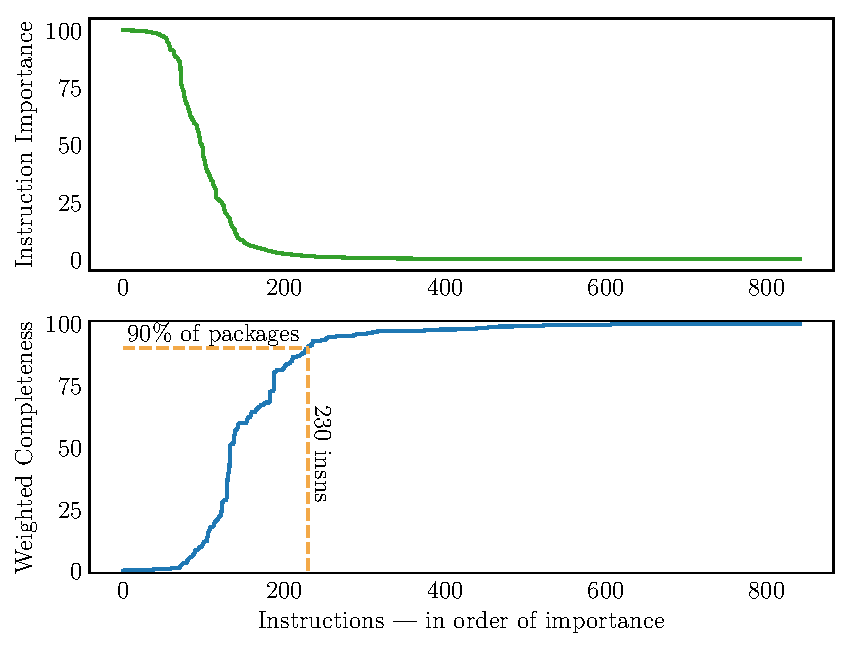
\includegraphics[width=0.5\linewidth]{figures/WCvMnem.pdf}
	\caption{ Instruction Importance (top): Distribution of instructions by percent of packages that need the instruction. Weighted completeness(bottom): What percent of packages can execute on a system that follows a greedy implementation strategy?}
	\label{fig:WCvMnem}
\end{figure}

Binary translation of a gargantuan ISA like Intel x86-64, which has
\textasciitilde{}3800 instructions, requires prioritizing development effort
on the most ``important'' instructions---trading completeness for simplicity
and a quicker development cycle.
For instance, the authors of VMware workstation describe an ``on-demand
implementation'' process, where the x86 binary translator focused on just the
instructions needed for a target OS; the entire ISA was never supported, and
guest OSes such as OS/2 did not work~\cite{bugnion-workstation}.
Similarly, Amit et al.~\cite{amit-161} showed that KVM cannot correctly
implement certain obscure x86 behaviors in a guest OS.
Prioritizing instruction support is a natural and ubiquitous engineering
trade-off. Some instructions appear in program binaries more frequently than
others, e.g., the \texttt{MOV} instruction (used to move data) is the most
common \texttt{x86-64} instruction. On the contrary, the \texttt{VFM\-ADD\-SD}
instruction, used to express a fused multiplication and addition operation, is
relatively rare. Further, many instructions perform similar operations, albeit
with subtle distinctions.

What, then, is the basis for assigning priority to instructions? Common
approaches include analyzing benchmark suites~\cite{SPEC2017-ab,Henning2006-ns,
bienia11benchmarking}, or execution traces collected in target
environments~\cite{elastictraces-axa}.
The ad-hoc nature of this approach leaves many useful questions unanswered:
Is the chosen test suite actually representative?
What is the path of least effort to support a new ISA in a software tool?
What minimum set of instructions must be implemented to run at least one
application? What instruction sub-set is sufficient to run the majority of
deployed applications?

To paraphrase Hennessy and Patterson~\cite{Patterson-textbook}, the best thing
to measure is what actually runs on the user's system.
This chapter will present and analyze a dataset collected from static analysis
of all x86-64 ELF binaries in the Ubuntu 16.04 GNU/Linux distribution.
We leverage package installation frequency, an approximation of a package's
importance to users, from Ubuntu and Debian popularity contest
data~\cite{ubuntu-popcon-tj,debian-popcorn-sb}, to infer the relative
importance of an instruction from the percentage of binaries on a given
system that contain that instruction.
We adapt metrics from a prior study of OS API compatibility~\cite{Tsai2016-zq},
specifically, \textit{instruction importance} --- the relative importance of
a given instruction, and \textit{weighted completeness} --- the completeness
of a system that implements a subset of the ISA.

Figure~\ref{fig:WCvMnem} is illustrative of the kinds of analysis our dataset
is useful for. The data presented in the figure shows that a small number of
instructions, about 30, are indispensable to all applications. The top 100
most important instructions are used by \texttildelow{}88\% of all packages.
Importance drops to 10\% by the 200~\textsuperscript{th} instruction, and 1\%
by the 240~\textsuperscript{th} instruction.

\noindent This chapter will present:
\begin{itemize}[noitemsep, topsep=0pt, leftmargin=1em, labelwidth=*, align=left]
\item An instruction occurrence dataset gathered using static analysis of
	9,337 open-source applications in the Ubuntu 16.04 repositories.
\item Evaluation of conventional wisdom about ISA usage.
\item An iterative plan for developing new tools that use the
	\texttt{x86-64} ISA.
\item Empirical validation of standard benchmarks.
\item An instruction occurrence data visualization tool, and the analysis framework used in this study are available at
	\url{http://x86instructionpop.com/}.
\end{itemize}

This chapter will be drawn from joint work~\cite{x86-systor} with Bhushan
Jain, Chia-che Tsai, Michael Ferdman and Donald E. Porter.